\documentclass[12pt,oneside,a4paper]{article}

% Pacotes básicos
\usepackage[utf8]{inputenc} % codificação de entrada
\usepackage[T1]{fontenc} % codificação da fonte
\usepackage[brazil]{babel} % idioma português
\usepackage{graphicx} % inclusão de imagens
\usepackage{amsmath,amsfonts,amssymb} % símbolos matemáticos
\usepackage{setspace} % controle de espaçamento
\usepackage{hyperref} % links clicáveis
\usepackage{geometry} % margens
\usepackage{titlesec} % formatação de títulos
\usepackage{subcaption}  % subfigure
\usepackage{booktabs}
\usepackage{xcolor}
\usepackage{tablefootnote}
\usepackage{indentfirst} %indent um novo parágrafo
\setlength{\parindent}{1.25cm} 
\definecolor{minhacor}{rgb}{1, 0, 0.5176}


% Margens
\geometry{left=3cm,right=2cm,top=3cm,bottom=2cm}

% Estilo de citação ABNT
\usepackage[alf]{abntex2cite}

% Espaçamento entre linhas
\onehalfspacing

% Início do documento
\begin{document}

% Capa
\begin{titlepage}
    \begin{center}
        \Large
        \textbf{FEA-USP}\\[1cm]
        \textbf{Avaliação de Políticas Sociais}\\[4cm]
        
        \textbf{\huge Impacto da extensão do direito de pensão alimentícia sobre a educação de mulheres jovens em união estável}\\[1cm]
        
        \large

        \textbf{Camila Machado, Giovanni Zanetti,  Hiaman Santos, Tuffy Issa }\\[6cm]
        
        \textbf{São Paulo}\\
        \textbf{2025}
    \end{center}
\end{titlepage}


% Sumário
\newpage
\tableofcontents
\newpage

% Introdução
\section{Introdução}

O desenvolvimento do presente trabalho foi orientado pela pergunta de pesquisa: ``\textit{Qual foi o impacto da extensão do direito à pensão alimentícia sobre a educação de mulheres jovens em união estável?}''. Para avaliar essa questão, explora-se a implementação da Lei nº 8.971/1994 \cite{brasil_lei8971_1994}, que estendeu os direitos de pensão alimentícia para casais em união consensual, o que era anteriormente concedido apenas para casamentos (ou seja, uniões legalmente formalizadas). A promulgação da Lei é tratada como uma variação institucional exógena, que afeta o \textit{outcome} de mulheres em uniões estáveis pelo canal de melhora de sua \textit{``fallback position''}, que é a ``melhor alternativa que um indivíduo dentro de uma relação marital teria se a cooperação dentro do casamento falhasse''\cite{agarwal1997bargaining}. 

A hipótese subjacente é de que, ao viabilizar uma fonte de renda para a parte que ficou em desvantagem econômica após o fim do relacionamento, haveria alguma influência sobre a decisão de investimento em capital humano para a parte desfavorecida, por meio da educação. Ainda que, sob o princípio constitucional de igualdade entre sexos, o legislador tenha assegurado ao companheiro e à companheira os mesmos direitos sob a Lei nº 8.971/1994, por razões históricas e sociais, considera-se que são as mulheres o grupo em desvantagem econômica após o relacionamento \cite{smock1999effect,gadalla2008impact}.  

Empregam-se as metodologias de pareamento por escore de propensão - ``\textit{propensity score matching}'' (PSM) - e diferença em diferenças - \textit{difference in differences} (DiD) -, com base em \citeonline{rangel2006alimony}, com o objetivo de estimar o efeito da política sobre mulheres em uniões consensuais. O grupo de controle utilizado é o de mulheres em casamentos formais, aliado a controles de características demográficas, regionais, sociais e de renda. Parte-se do pressuposto de que casais em condição de casamento formal não foram afetados pela mudança institucional, uma vez que os direitos assegurados pela Lei 8.971/1994 já estavam previamente assegurados a esse grupo. Dessa forma, não haveria incentivos para alterar seu status jurídico de união.

Os microdados para os indivíduos foram extraídos da Pesquisa Nacional por Amostra de Domicílios (PNAD) para os anos de 1992, 1993 e 1995, permitindo, assim, comparar os resultados educacionais de mulheres em união estável antes e depois da implementação da Lei nº 8.971/1994.

\subsection{Contexto legal}

A Lei nº 8.971/1994 modificou a legislação brasileira ao ampliar os direitos de pensão previstos na Lei nº 5.478/1968 \cite{brasil_lei5478_1968}, dados alguns critérios de elegibilidade. Com essa mudança, a companheira comprovada de homem solteiro, separado judicialmente, divorciado ou viúvo, passou a ter direito à pensão alimentícia, desde que demonstrada a convivência por mais de cinco anos. A exigência de tempo mínimo de convivência não se aplicava quando, da união estável, tivesse surgido prole. Ainda de acordo com tal norma, o direito à pensão permanecia válido até que a companheira constituísse nova união e enquanto continuasse comprovando necessidade. 

A alteração do aparato normativo foi feito em um contexto em que as uniões estáveis (``concubinato'', termo utilizado pelo legislador) cresciam no Brasil. Como aponta \citeonline{rangel2006alimony}, a proporção de uniões informais aumentou de 16.6\% para 28\% em 1995, com mais da metade dessas uniões consensuais durando mais de 6 anos. O autor sugere que tal aumento pode ser interpretado como uma forma de compensar a tendência de aumento no número de divórcios e de queda dos casamentos formais. Antes da Lei 8.971/1994, os tribunais indeferiam pedidos de pensão alimentícia para casos de uniões informais. Isso porque a jurisprudência considerava que os ``concubinos'' não eram ``nem parentes, nem cônjunges, não havendo amparo legal para que pudessem exigir alimentos, um do outro'' \cite{wald1995lei}.


\section{Dados}

Os microdados utilizados foram extraídos da Pesquisa Nacional por Amostra de Domicílios (PNAD), conduzida pelo Instituto Brasileiro de Geografia e Estatística (IBGE) nos anos de 1992, 1993 e 1995.\footnote{A coleta de dados não ocorreu no ano de 1994 devido a problemas orçamentários, por este motivo o ano de introdução da nova legislação não consta na base de dados.} O mês de referência para a coleta de dados é o mês de setembro de cada um dos anos, e o modelo fixo do questionário aplicado permite comparar os dados para cada um dos recenseamentos. Entre as informações acessadas na PNAD estão: as características da demografia domiciliar, renda, oferta de trabalho e investimentos escolares. Especificamente para os anos selecionados, são incluídas informações adicionais sobre a condição de coabitação e casamentos formais. A amostra anual consiste de aproximadamente 45.000 observações em casais adultos e 65.000 observações sobre crianças de 5 a 17 anos de idade. A amostra permite permite a condução de análises em contextos variados, contribuindo para a verificação da plausibilidade das hipóteses subjacentes à estratégia de identificação causal. 

Com o objetivo de analisar o efeito da política sobre os anos estudados das mulheres em união estável, ampliou-se a amostra utilizada por \cite{rangel2006alimony}. Desta forma, optou-se por analisar o efeito da política sobre o grupo de mulheres mais jovens, entre 15 e 24 anos de idade, por se tratar da faixa etária mais propensa a abandonar os estudos após a maternidade. Esta seleção visa a captar os possíveis efeitos da introdução da nova política de pensão alimentícia sobre a permanência escolar, em decorrência da redução da substituição de educação por atividades no mercado de trabalho formal ou doméstico, dada a garantia de apoio financeiro.

Assim, para a definição do grupo tratado, selecionou-se, na amostra, as mulheres de 15 a 24 anos, em união não formal - seja união consensual ou apenas religiosa - identificadas como responsáveis ou cônjuges do responsável pelo domicílio. O grupo de controle, por sua vez, abrangeu mulheres de 15 a 24 anos, identificadas em casamentos com registro civil ou com registro civil e religioso, que foram apontadas como responsáveis ou como cônjuges do responsável pelo domicílio.  

A Tabela \ref{tab:desc} apresenta as características descritivas da base de dados utilizada para a análise do efeito da política, isto é, após a seleção dos grupos de mulheres casadas e em união estável. Nota-se que o grupo de mulheres tratadas corresponde a 45\% do total da amostra de mulheres em união estável e casadas. Em relação às características socioeconômicas, destaca-se que 55\% das mulheres são brancas ou amarelas, e a idade média da amostra é de 21 anos, com desvio padrão de 2.4 anos. Em termos de escolaridade, a amostra apresenta média de 6.6 anos de estudo. Em relação ao curso que frequentam, para essa amostra, a média seria equivalente ao atual Ensino Médio. A renda domiciliar média é de Cr\$ 173,000. A proporção de mulheres que declararam receber pensão alimentícia é praticamente nula (0.00), com um pequeno número de casos positivos (desvio-padrão de 0.05). Com relação à composição familiar, as mulheres têm, em média, 1.17 filhos residindo em seus domicílios, sendo aproximadamente 0.57 filhos homens e 0.55 filhas mulheres.

\begin{table}

\caption{Estatísticas descritivas ponderadas}
\centering
\label{tab:desc}
\begin{tabular*}{\textwidth}{@{\extracolsep{\fill}}lcccc}
\toprule
  & Média & DP & Min & Max\\
\midrule
Tratamento & 0.45 & 0.50 & 0 & 1\\
Sexo (fem = 1) & 1.00 & 0.00 & 1 & 1\\
Cor/Raça (PPI = 0) & 0.55 & 0.50 & 0 & 1\\
Curso Mais Elevado & 4.22 & 0.56 & 0 & 9\\
Idade & 21.04 & 2.41 & 15 & 24\\
\addlinespace
Anos de Estudo & 6.61 & 3.37 & 1 & 17\\
Última série concluída & 4.47 & 2.00 & 1 & 9\\
Curso que frequenta & 2.48 & 1.65 & 0 & 9\\
Renda dom. per capita \tablefootnote{Os rendimentos foram reportados em moedas diferentes para cada um dos anos da amostra} & 173,221.66 & 269,756.48 & 0 & 9,549,387\\
Pensão (sim = 1) & 0.00 & 0.05 & 0 & 1\\
\addlinespace
Grupo CBO & 4.34 & 2.58 & 0 & 8\\
Filhos Homens (dom.) & 0.57 & 0.72 & 0 & 12\\
Filhos Mulheres (dom.) & 0.55 & 0.71 & 0 & 6\\
Total de filhos & 1.17 & 1.00 & 0 & 13\\
\bottomrule
\end{tabular*}
\end{table}

 
Devido a preocupação de que os rendimentos não sejam comparáveis entre os anos, apresentamos uma a Tabela \ref{tab:renda_dom_pc} com estatísticas simples, a fim de verificarmos que a variável de rendimento domiciliar per capita foi padronizada entre os anos da pesquisa.
\begin{table}[ht]
\centering
\small  % ou \footnotesize
\caption{Estatísticas da renda domiciliar per capita}
\label{tab:renda_dom_pc}
\begin{tabular}{rrrrrrr}
  \hline
ano & n & Média & Mediana & DP & Mínimo & Máximo \\ 
  \hline
92 & 333,205 & 254,596.16 & 132,500.00 & 481,558.27 & 0.00 & 41,833,333.33  \\ 
93 & 338,858 & 218,563.22 & 111,363.64 & 438,577.80 & 0.00 & 41,833,333.33 \\ 
95 & 351,780 & 201,692.53 & 100,273.25 & 434,272.26 & 0.00 & 41,833,333.33  \\ 
  \hline
\end{tabular}
\end{table}

% Metodologia
\section{Metodologia}

\subsection{Fundamentação teórica}

A metodologia de \textit{difference in differences} (DiD) é uma técnica quase-experimental empregada para estimar o efeito causal de uma intervenção. Seu funcionamento baseia-se na comparação da mudança no resultado de interesse ao longo do tempo para um grupo que recebeu o tratamento, com a mudança no mesmo resultado para um grupo comparável que não foi exposto à intervenção, que é o grupo controle. O método isola o impacto específico da intervenção, controlando simultaneamente por tendências temporais comuns que afetariam ambos os grupos e por diferenças fixas e pré-existentes entre eles. 

Em \citeonline{rangel2006alimony} o método é utilizado para comparar casais em união consensual (o grupo de tratamento, afetado pela extensão dos direitos de pensão alimentícia) com casais formalmente casados (o grupo de controle, não diretamente afetado por essa legislação específica), tanto antes quanto depois da implementação da lei. O objetivo é ``compensar os efeitos de quaisquer fatores de confusão'' que poderiam, de outra forma, mascarar o verdadeiro impacto da política.

Já o \textit{Propensity Score Matching} (PSM) é uma técnica utilizada para reduzir o viés de seleção em estudos observacionais. Seu objetivo é criar um grupo de controle que seja ``balanceado'' em relação ao grupo de tratamento em termos de características observáveis, o que é alcançado estimando-se a probabilidade de um indivíduo receber o tratamento, dado seu vetor de covariadas observadas, formalmente expressa como $E(X_i)=P(T_i=1 \mid X_i)$. Em seguida, indivíduos com escores de propensão similares são pareados entre os grupos de tratamento e controle.

A metodologia pode ser representada pelo modelo teórico abaixo:

$$Y_\text{it} = \alpha_0 + t_t\cdot \alpha_1 + T_i\cdot \alpha_2 + X_i\beta + (T_i \cdot t_t)\cdot \tau + \eta_\text{it}$$ 
onde: 

\begin{itemize}
    \item $t_t$ é uma \textit{dummy} que indica se o período em questão é pré ou pós-tratamento;
    \item $T_i$ é uma \textit{dummy} que indica se o indivíduo pertence ao grupo de tratamento ou de controle;
    \item $(T_i\cdot t_t)$ é o termo de interação, que recebe valor 1 se o indivíduo pertence ao grupo de tratamento ou de controle, antes ou depois de o tratamento ter sido implementado;
    \item $X_i$ é um vetor de características observáveis.
\end{itemize}

\subsubsection{Estratégia de identificação}

Considerando a amostra dos indivíduos \textbf{pareados}, a identificação do efeito causal do tratamento envolve a hipótese de que seus \textit{outcomes} seguiriam \textbf{tendências paralelas} na ausência da Lei 8.971/1994, ou seja:

$$\mathbb{E}[Y_i(0) \mid T_i = 1, t_t = 1, X_i] - \mathbb{E}[Y_i(0) \mid T_i = 1, t_t=0, X_i] = $$
$$\mathbb{E}[Y_i(0) \mid T_i = 0, t_t =1, X_i] - \mathbb{E}[Y_i(0) \mid T_i = 0, t_t = 0, X_i]$$

Para o PSM, a suposição de ignorabilidade condicional é fundamental: condicional às covariadas observadas, a atribuição ao grupo de tratamento (mulheres em união estável) é independente do resultado potencial na ausência do tratamento. Em outras palavras, após o pareamento, não há características observáveis que tornem um indivíduo mais propenso a estar em união estável e que também afetem o resultado de educação independentemente da lei. Uma vez que nossa amostra é balanceada em termos das características selecionadas (graças ao PSM), indivíduos pareados têm uma probabilidade similar de pertencer ao grupo de tratamento, mitigando o viés de seleção baseado nessas covariadas.

No contexto da combinação de PSM com DiD, a principal preocupação com a violação dessa hipótese de ignorabilidade estaria em cenários onde a decisão de manter o status de união (formal ou consensual) pudesse ser influenciada pela expectativa da nova lei e essa influência fosse diferente para os grupos de tratamento e controle, afetando também seus resultados educacionais de forma distinta. No entanto, como os direitos conferidos às uniões consensuais pela Lei nº 8.971/1994 já existiam para indivíduos formalmente casados, é plausível assumir que a lei não incentivaria mulheres casadas a mudar seu status para união estável. Essa ausência de um ``incentivo'' para o grupo de controle alterar seu status em resposta à lei reforça a premissa de que as diferenças observadas pós-lei são atribuíveis ao tratamento e não a decisões estratégicas relacionadas ao status civil em decorrência da legislação.

Com o exposto acima, estima-se, no presente trabalho, o parâmetro \textit{Average Treatment Effect on the Treated} (ATT), que reflete o efeito do estabelecimento da Lei 8.971/1994 sobre o nível educacional de mulheres jovens pertencentes à uniões consensuais não-formais.

$$ATT = \mathbb{E}[Y_i(1) - Y_i(0) \mid T_i = 1, t_t = 1, X_i]$$

A avaliação do impacto da política sobre a escolaridade das mulheres jovens foi feita por meio da combinação de dois métodos econométricos, o \textit{Propensity Score Matching} (PSM) e \textit{Difference-in-Differences} (DiD).

\subsection{Aplicação - PSM}

Para o cálculo do \textit{PSM}, aplicou-se a seguinte formula para calcular os \textit{scores} de cada indivíduo:

$$ T_i = Idade_i + CorBA_i + UF_i + FH_i + FM_i + RC_i + Filhos_i $$

Onde, \(T_i\) é referente à condição de tratamento da mulher, assumindo valor de 1 ou 0; \(Idade_i\) é a variável de idade; \(CorBA_i\) é a \textit{dummy} quanto à cor/raça do indivíduos, assumindo valor igual a 1 para brancos/amarelos e 0 para PPI; \(FH_i\) é uma variável \textit{dummy} para a presença de filhos homens no domicílio; \(FM_i\) é \textit{dummy} para a presença de filhas mulheres no domicilio; \(RC_i\) é o valor da renda per capita do domicílio; \(UF_i\) é referente à Unidade Federativa do domicílio; \(Filhos_i\) é o total de filhos do indivíduo. A partir destas variáveis, então, buscou-se realizar o \textit{matching}.

\subsection{Aplicação - DiD}

Extraído os \textit{scores} através do \textit{PSM}, segue-se a análise da política para a estimação quanto ao seu efeito. Com este objetivo, aplicou-se o método de \textit{DID} com a seguinte equação:

$$ Anos\_Estudo_i = \beta_0 + \beta_1D + \beta_2T_i + \beta_3(D \times T_i) + X_i + \lambda_{i,t} + \varepsilon_i$$

A variável dependente são os anos de estudo de cada indivíduo, representada por \(Anos\_Estudo_i\). Ademais, as variáveis independentes são: \(D\), uma \textit{dummy} indicando o ano de 1995, sendo este o período posterior à introdução da nova política; \(T_i\), a indicação de tratamento; o vetor de características do indivíduo \(X_i\), composto pela raça, idade e número de filhos; \(\lambda_{i,t}\) é referente ao efeito fixo no qual a UF e o ano amostral foram interagidos. Assim, a partir desta equação, o efeito da política será apresentado pelo coeficiente \(\beta_3\), enquanto o coeficiente \(\beta_1\) indica o período pós-tratamento, \(\beta_2\) a inclinação para o grupo tratado e \(\beta_0\) o intercepto. 


% Análise e Discussão dos Resultados
\section{Resultados}
\subsection{Pareamento}

Realizado o pareamento a partir das características demográficas, regionais, sociais e de renda das mulheres, os resultados estão expostos na Tabela \ref{tab:descriptive}. Os resultados de destaque são referentes ao tamanho efetivo da amostra (\textit{effective sample size} (ESS)), refletindo o pareamento utilizando o peso amostral de cada observação da PNAD. Dentre todos os três painéis da Tabela \ref{tab:descriptive} destaca-se que todos os tratamentos foram pareados, sem que houvesse perda ou descarte de observações dentro do grupo de tratados.

\begin{table}[htbp]
\centering
\caption{Resultados de Pareamento}
\label{tab:descriptive}
\begin{tabular*}{\textwidth}{@{\extracolsep{\fill}}lcc}
\toprule
\textbf{Categoria} & \textbf{Controles} & \textbf{Tratados} \\
\midrule
\addlinespace[0.5ex]
\multicolumn{3}{@{}l}{\textbf{Painel A: Pareamento 1992}} \\

All (ESS) & 3729.659 & 2517.267\\
All & 4385.000 & 3041.000\\
Matched (ESS) & 1190.516 & 2517.267\\
Matched & 1990.000 & 3041.000\\
Unmatched & 2395.000 & 0.000\\
\addlinespace
Discarded & 0.000 & 0.000\\



\\
\addlinespace[1ex]
\multicolumn{3}{@{}l}{\textbf{Painel B: Pareamento 1993}} \\

All (ESS) & 3022.163 & 2354.72\\
All & 3527.000 & 2858.00\\
Matched (ESS) & 1162.231 & 2354.72\\
Matched & 1780.000 & 2858.00\\
Unmatched & 1747.000 & 0.00\\
\addlinespace
Discarded & 0.000 & 0.00\\


\\
\addlinespace[1ex]
\multicolumn{3}{@{}l}{\textbf{Painel C: Pareamento 1995}} \\

All (ESS) & 3022.163 & 2354.72\\
All & 3527.000 & 2858.00\\
Matched (ESS) & 1162.231 & 2354.72\\
Matched & 1780.000 & 2858.00\\
Unmatched & 1747.000 & 0.00\\
\addlinespace
Discarded & 0.000 & 0.00\\


\\
\midrule
\bottomrule
\end{tabular*}        
\end{table}

Ademais, um teste de médias foi realizado para o paramento de cada um dos períodos. O resultado final está expresso na Figura \ref{fig:match}. Nota-se que, para o pareamento de 1992 (Figura \ref{fig:match_92}), apenas duas variáveis apresentaram diferença significativa entre os grupos, quais sejam, a diferença de Idade e de Renda per Capita. Por outro lado, para os outros dois períodos de pareamento, nota-se que apenas a idade dos indivíduos apresenta uma diferença estatisticamente significativa (Figuras \ref{fig:match_93} e \ref{fig:match_95}). Apesar dessa diferença observada, os resultados gerais apontam para um \textit{PSM} que introduziu maior comparabilidade entre o grupo de tratamento e controle, já que todas as demais diferenças, antes significativas, passaram a ser não significativas dentro de cada um dos anos.


\begin{figure}[ht]
    \centering
    \caption{Pareamentos}
    \label{fig:match}

    \begin{subfigure}[b]{0.5\linewidth}
        \centering
          \caption{Pareamento - 1992}
        \label{fig:match_92}
        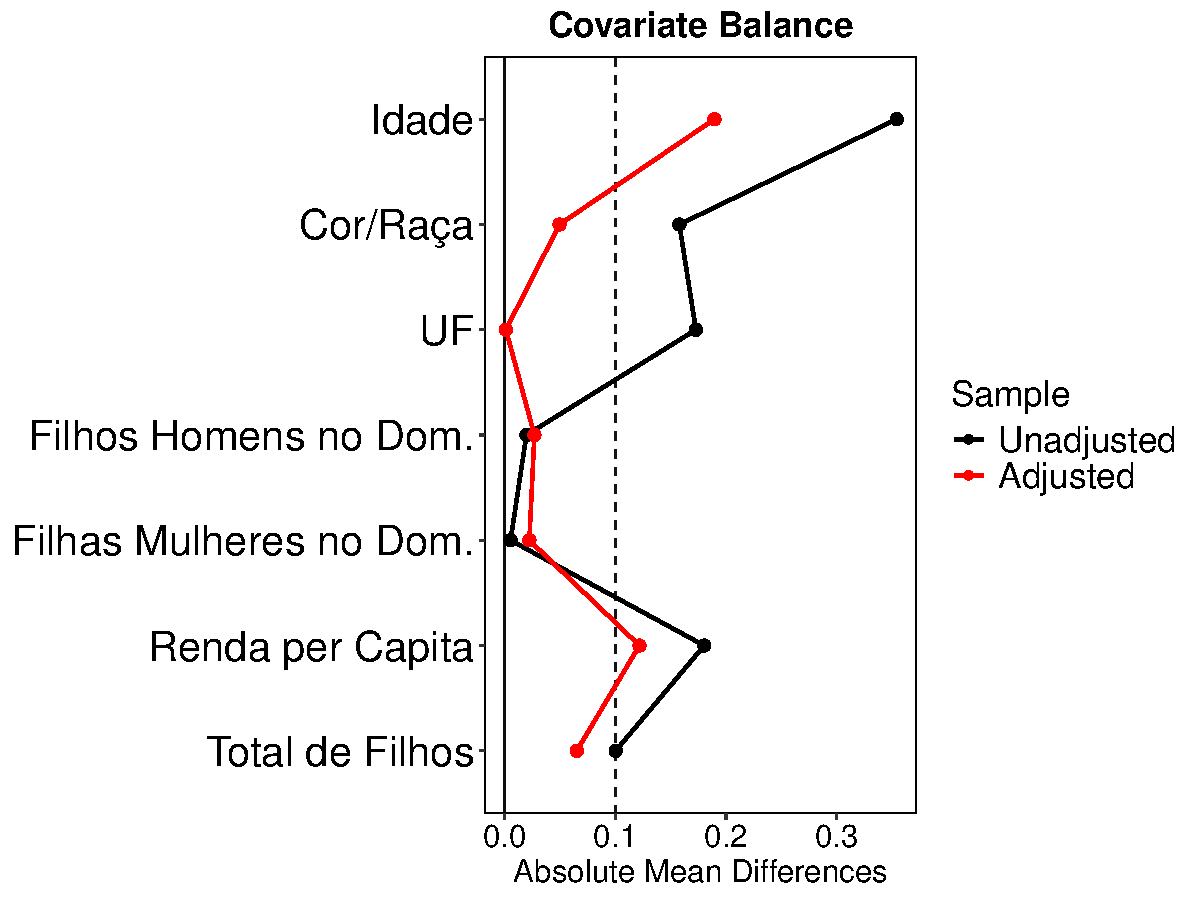
\includegraphics[width=\linewidth]{figuras/balance/1992_matchit_summary_love_plot.pdf}
    \end{subfigure}

    \begin{subfigure}[b]{0.5\linewidth}
        \centering
         \caption{Pareamento - 1993}
        \label{fig:match_93}
        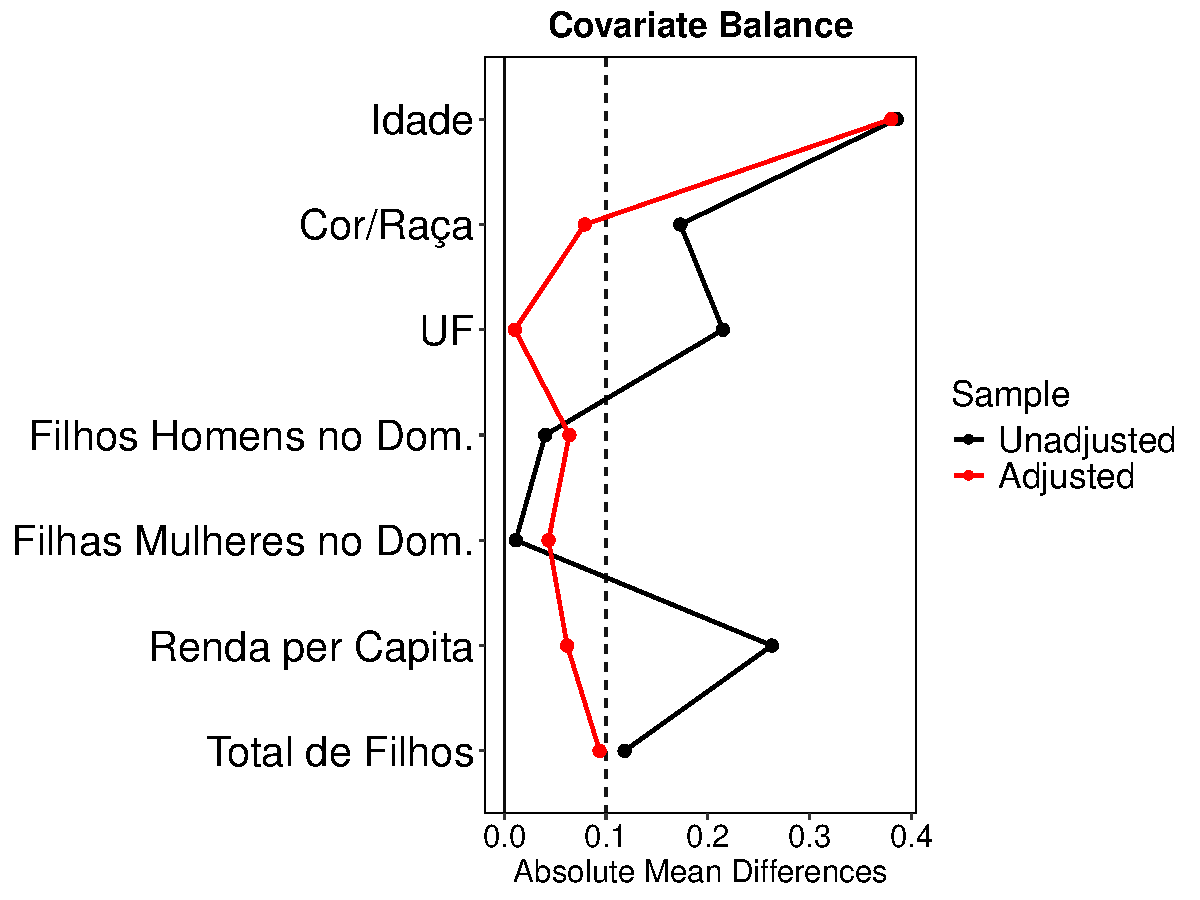
\includegraphics[width=\linewidth]{figuras/balance/1993_matchit_summary_love_plot.pdf}
       
    \end{subfigure}%
    \begin{subfigure}[b]{0.5\linewidth}
        \centering
         \caption{Pareamento - 1995}
        \label{fig:match_95}
        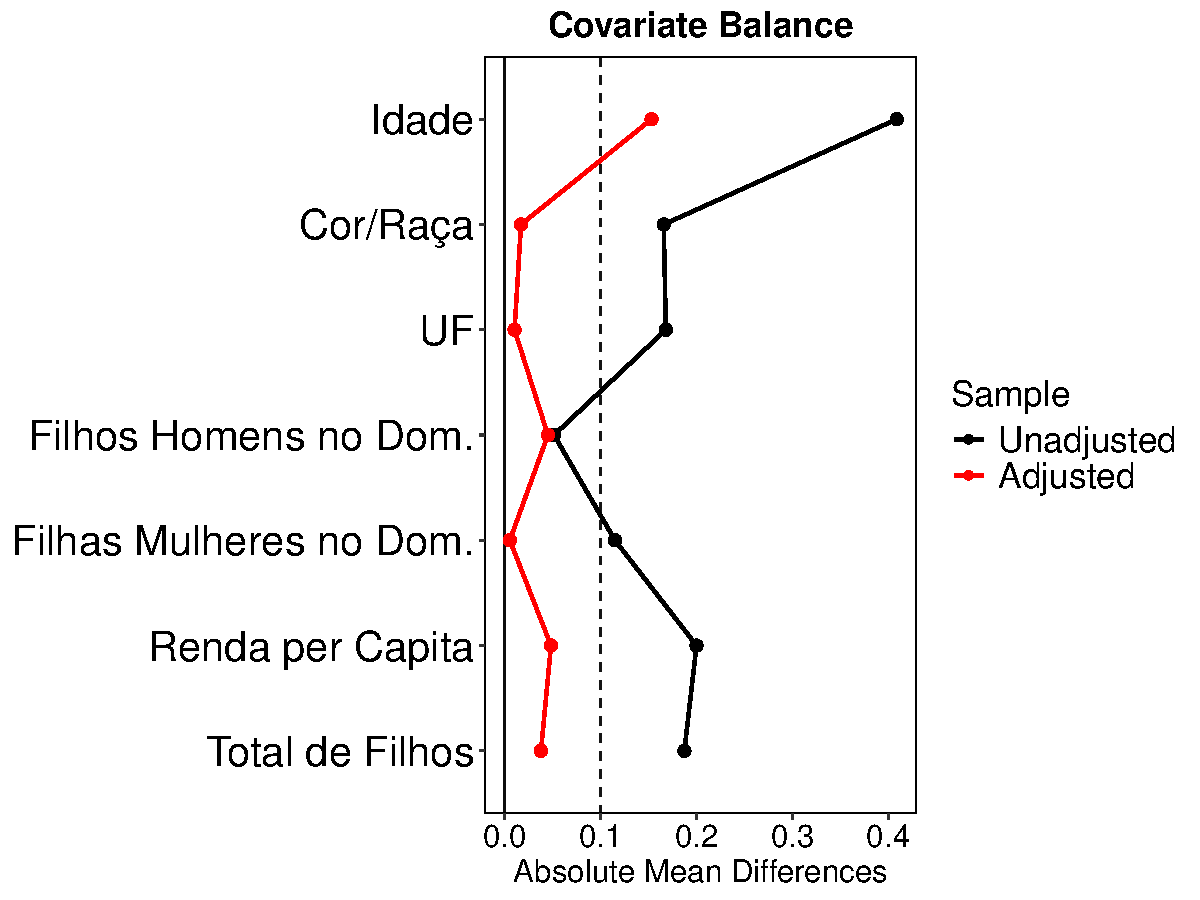
\includegraphics[width=\linewidth]{figuras/balance/1995_matchit_summary_love_plot.pdf}
    \end{subfigure}

\end{figure}

\subsection{Efeito sobre educação}

Os resultados da estimação principal estão expostos na Tabela \ref{tab:dif_principal}. O coeficiente de interesse, associado à interação entre o grupo de tratamento e o período pós-política (Tratamento × D), não apresentou significância estatística em nenhuma das três especificações utilizadas. Mesmo no modelo mais completo, com efeitos fixos por UF e ano, o coeficiente estimado foi negativo e não estatisticamente diferente de zero.


\begin{table}[htbp]
   \caption{\label{tab:dif_principal} Resultados Principais}
   \centering
\begin{tabular*}{\textwidth}{@{\extracolsep{\fill}}lccc}
      \tabularnewline \midrule \midrule
      Dependent Variable: & \multicolumn{3}{c}{Anos de Estudo}\\
      Model:                          & (1)            & (2)            & (3)\\  
      \midrule
      \emph{Variables}\\
      Tratamento                      & -1.116$^{***}$ & -1.125$^{***}$ & -0.8376$^{***}$\\   
                                      & (0.0713)       & (0.0691)       & (0.0663)\\   
      $D$                       & -0.0223        &                &   \\   
                                      & (0.1096)       &                &   \\   
      Tratamento $\times$ $D$   & 0.0656         & 0.0614         & -0.0858\\   
                                      & (0.1256)       & (0.1205)       & (0.1133)\\   
      Total de Filhos                 &                &                & -0.7272$^{***}$\\   
                                      &                &                & (0.0268)\\   
      Cor/Raça                        &                &                & 0.5867$^{***}$\\   
                                      &                &                & (0.0538)\\   
      Idade                           &                &                & 0.2687$^{***}$\\   
                                      &                &                & (0.0108)\\   
      \midrule
      \emph{Fixed-effects}\\
      UF$	\times$Ano                   &                & Yes            & Yes\\  
      \midrule
      \emph{Fit statistics}\\
      Observations                    & 14,621         & 14,621         & 14,621\\  
      R$^2$                           & 0.03672        & 0.08445        & 0.17791\\  
      Within R$^2$                    &                & 0.03913        & 0.13722\\  
      \midrule \midrule
      \multicolumn{4}{l}{\emph{Heteroskedasticity-robust standard-errors in parentheses}}\\
      \multicolumn{4}{l}{\emph{Signif. Codes: ***: 0.01, **: 0.05, *: 0.1}}\\
   \end{tabular*}
\end{table}




Ademais, a Tabela \ref{tab:dif_ano} apresenta uma análise com interações por ano, com 1992 como referência. Os coeficientes associados aos anos de 1993 e 1995 também não apresentaram significância estatística, mesmo na especificação mais robusta. O fato de não haver variação significativa nas diferenças entre grupos ao longo do tempo reforça a hipótese de que a política não alterou substancialmente o grau de educação das mulheres tratadas dentro da janela temporal analisada. 
Os efeitos significativos ao longo das especificações foram a penalidade aos anos de educação associada ao número total de filhos, idade e cor/raça. Tanto cor/raça quanto idade apresentam coeficientes positivos, sugerindo que mulheres mais velhas e brancas/amarelas possuem em média mais anos de educação. Por fim, o coeficiente associado ao número total de filhos indica que, em média, cada filho a mais está relacionado a uma redução de 0.73 anos de estudo das mulheres jovens.



\begin{table}[htbp]
   \caption{\label{tab:dif_ano} Resultados por ano}
   \centering
\begin{tabular*}{\textwidth}{@{\extracolsep{\fill}}lccc}
      \tabularnewline \midrule \midrule
      Dependent Variable: & \multicolumn{3}{c}{Anos de Estudo}\\
      Model:                            & (1)            & (2)            & (3)\\  
      \midrule
      \emph{Variables}\\
      Tratamento                        & -1.154$^{***}$ & -1.032$^{***}$ & -0.8220$^{***}$\\   
                                        & (0.0717)       & (0.0956)       & (0.0917)\\   
      Tratamento $\times$ ano $=$ 1993  & 0.0922         & -0.1951        & -0.0329\\   
                                        & (0.0726)       & (0.1383)       & (0.1298)\\   
      Tratamento $\times$ ano $=$ 1995  & 0.0878         & -0.0316        & -0.1015\\   
                                        & (0.0707)       & (0.1374)       & (0.1298)\\   
      Total de Filhos                   &                &                & -0.7271$^{***}$\\   
                                        &                &                & (0.0267)\\   
      Cor/Raça                          &                &                & 0.5866$^{***}$\\   
                                        &                &                & (0.0538)\\   
      Idade                             &                &                & 0.2686$^{***}$\\   
                                        &                &                & (0.0108)\\   
      \midrule
      \emph{Fixed-effects}\\
      UF$\times$Ano                     &                & Yes            & Yes\\  
      \midrule
      \emph{Fit statistics}\\
      Observations                      & 14,621         & 14,621         & 14,621\\  
      R$^2$                             & 0.03682        & 0.08464        & 0.17791\\  
      Within R$^2$                      &                & 0.03934        & 0.13723\\  
      \midrule \midrule
      \multicolumn{4}{l}{\emph{Heteroskedasticity-robust standard-errors in parentheses}}\\
      \multicolumn{4}{l}{\emph{Signif. Codes: ***: 0.01, **: 0.05, *: 0.1}}\\
   \end{tabular*}
\end{table}






% Considerações Finais
\section{Conclusões}

Os resultados obtidos não indicam um impacto estatisticamente significativo da Lei nº 8.971/1994 sobre a escolaridade de mulheres jovens em união estável, ao menos no curto prazo após a promulgação da lei. Embora a teoria econômica e sociológica fundamente a expectativa de que o fortalecimento da "\textit{fallback position}" da mulher, via direitos de pensão alimentícia, possa levar a maiores investimentos em capital humano, não se encontrou evidência empírica suficiente para confirmar essa hipótese no contexto analisado.

A estratégia de identificação adotada, que combina \textit{propensity score matching} com Diferença-em-Diferenças, depende de pressupostos fortes. Em especial, a validade do DiD requer que os grupos de tratamento e controle apresentem tendências paralelas na ausência da política, e ainda que a análise por ano aponte para variações não significativas nos períodos pré e pós-tratamento, a ausência de dados para anos anteriores a 1992 limita a apresentação de evidências que a tornem mais crível. Ainda assim, o pareamento com \textit{propensity score} oferece suporte adicional à validade da identificação.

A fim de aprimorar a análise, seriam úteis dados que permitissem seguir os mesmos indivíduos ao longo do tempo. Informações sobre acesso efetivo aos benefícios da pensão (e não apenas a elegibilidade legal), também, poderiam elucidar melhor os mecanismos em questão. Além disso, uma janela temporal mais ampla poderia capturar efeitos de médio e longo prazo, especialmente se a resposta do comportamento educacional ao novo arcabouço legal for defasada. Trabalhos futuros podem explorar heterogeneidades no impacto da política por faixa de renda e região, bem como investigar interações com outras políticas públicas voltadas à proteção social das mães, com dados administrativos vinculados a registros judiciais ou a programas sociais como o Bolsa Família.


% Referências
\newpage
\bibliographystyle{abntex2-alf}
\bibliography{referencias}


\end{document}

